\section{Geriausio modelio įvertinimas}
\label{sec:geriausias_modelis}

Geriausias modelis abiem užduotims parinktas iš visų $17$ tyrimų variantų pagal didžiausią validavimo tikslumą ir mažiausią validavimo paklaidą (žr.~\ref{sec:tyrimo_rezultatai} sk.). Abiejose užduotyse laimėjo \textit{Batch Normalization} konfigūracija (\texttt{use\_batch\_norm}~$=\texttt{True}$) su numatytaisiais hiperparametrais.

Geriausias modelis perduodamas \texttt{evaluate\_best\_model} funkcijai, kuri:
\begin{enumerate}
    \item Iš naujo apmoko tinklą $20$ epochų – vaizdams su didesniu pošaliu (\texttt{subset\_ratio}~$=0{,}5$, $2\,958$ vaizdai vietoj $1\,182$); laiko eilutėms aibė lieka ta pati.
    \item Įvertina ant testavimo aibės.
    \item Sugeneruoja klasifikavimo matricą ir $30$ pavyzdinių spėjimų sąrašą (žr.~\ref{sec:pavyzdziu_klasifikacija} sk.).
\end{enumerate}

\begin{table}[H]
    \centering
    \caption{Geriausio modelio testavimo rezultatai abiem užduotims.}
    \begin{tabular}{|l|c|c|c|c|}
        \hline
        Užduotis & Klasių & Konfigūracija & \texttt{test\_acc} & \texttt{test\_loss} \\
        \hline
        Vaizdai (\textit{Muffin vs. Chihuahua})       & $2$  & \texttt{ImageCNN} su BN     & $\mathbf{0{,}8970}$ & $0{,}3292$ \\
        \hline
        Laiko eilutės (\textit{CMU Keystroke})         & $30$ & \texttt{KeystrokeCNN} su BN & $\mathbf{0{,}9167}$ & $0{,}3881$ \\
        \hline
    \end{tabular}
    \label{tab:best_model_summary}
\end{table}


\subsection{Vaizdų geriausias modelis}
\label{subsec:geriausias_vaizdai}

Galutinis modelis: \texttt{ImageCNN} su \texttt{(32, 64, 128)} filtrais, \textit{ReLU} aktyvacija, \texttt{Dropout}~$=0$, \textit{Adam} optimizatoriumi, \texttt{use\_batch\_norm}~$=\texttt{True}$. Po $20$ apmokymo epochų pasiekta:
\begin{itemize}
    \item Mokymo aibėje – $\texttt{train\_acc}=0{,}9942$, $\texttt{train\_loss}=0{,}0194$.
    \item Validavimo aibėje – $\texttt{val\_acc}=0{,}9133$ (geriausia $19$-a epocha).
    \item \textbf{Testavimo aibėje – $\texttt{test\_acc}=0{,}8970$, $\texttt{test\_loss}=0{,}3292$.}
\end{itemize}

\begin{figure}[H]
    \centering
    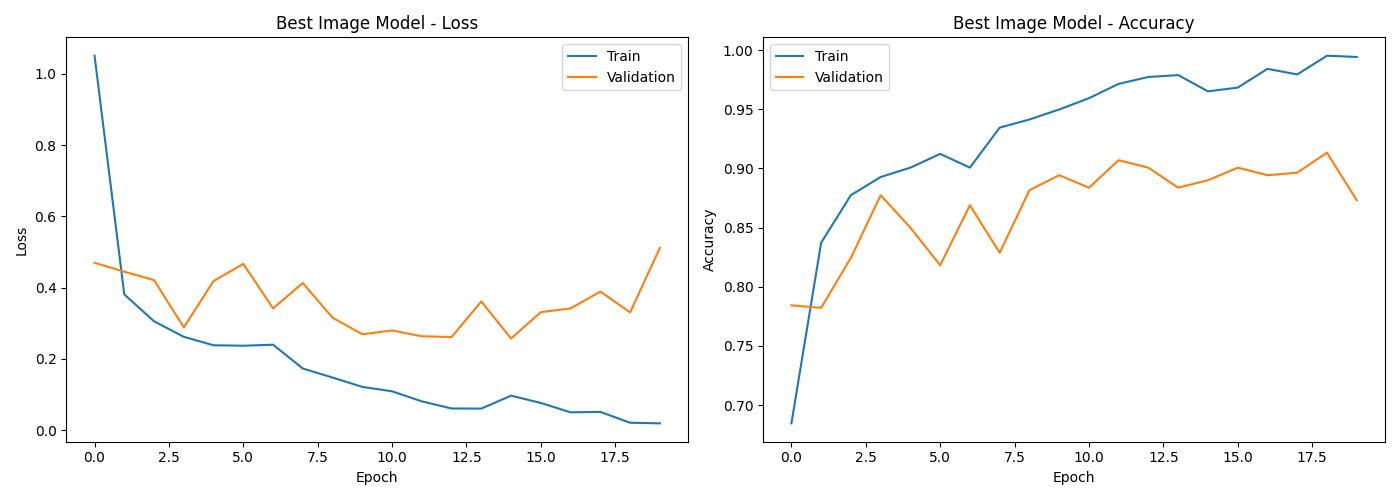
\includegraphics[width=0.9\linewidth]{3Lab/results/best_model/image/history.png}
    \caption{Vaizdų geriausio modelio mokymo ir validavimo metrikos}
    \label{fig:geriausias_image_history}
\end{figure}

\begin{figure}[H]
    \centering
    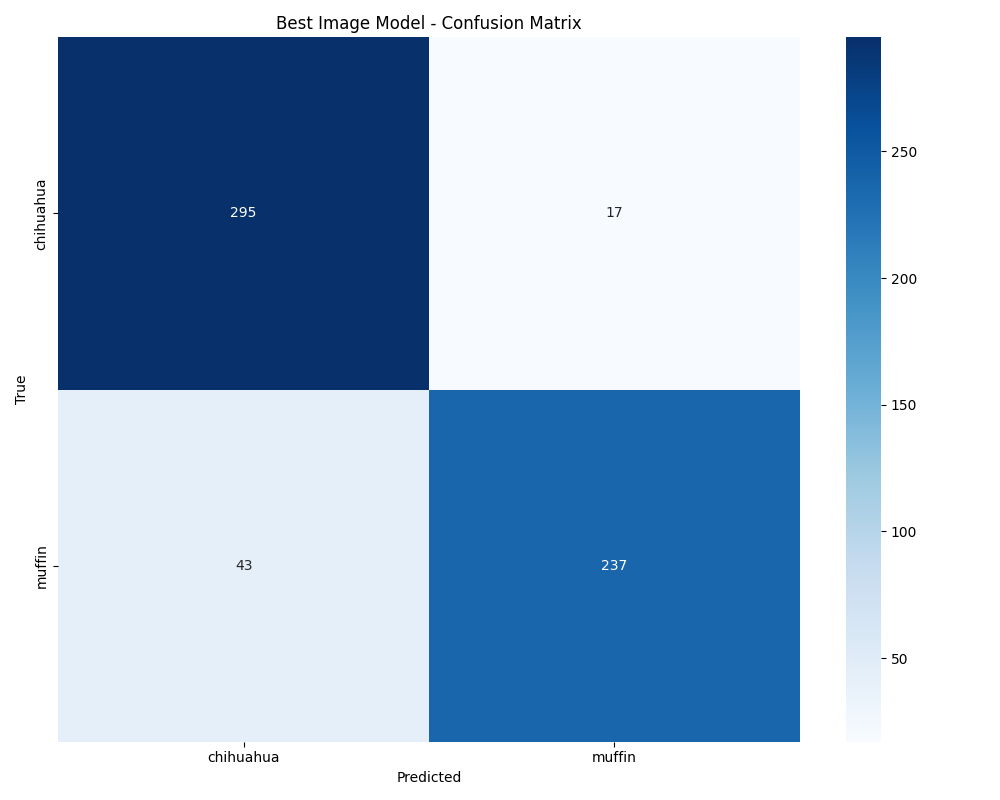
\includegraphics[width=0.6\linewidth]{3Lab/results/best_model/image/confusion_matrix.png}
    \caption{Vaizdų geriausio modelio klasifikavimo matrica (\textit{confusion matrix}) testavimo aibėje}
    \label{fig:geriausias_image_cm}
\end{figure}

\subsection{Laiko eilučių geriausias modelis}
\label{subsec:geriausias_keystroke}

Galutinis modelis: \texttt{KeystrokeCNN} su \texttt{(64, 128)} filtrais, \textit{ReLU} aktyvacija, \texttt{Dropout}~$=0$, \textit{Adam} optimizatoriumi, \texttt{use\_batch\_norm}~$=\texttt{True}$. Po $20$ apmokymo epochų pasiekta:
\begin{itemize}
    \item Mokymo aibėje – $\texttt{train\_acc}=0{,}9990$, $\texttt{train\_loss}=0{,}0372$.
    \item Validavimo aibėje – $\texttt{val\_acc}=0{,}9167$ (geriausia $18$-a epocha).
    \item \textbf{Testavimo aibėje – $\texttt{test\_acc}=0{,}9167$, $\texttt{test\_loss}=0{,}3881$.}
\end{itemize}

\begin{figure}[H]
    \centering
    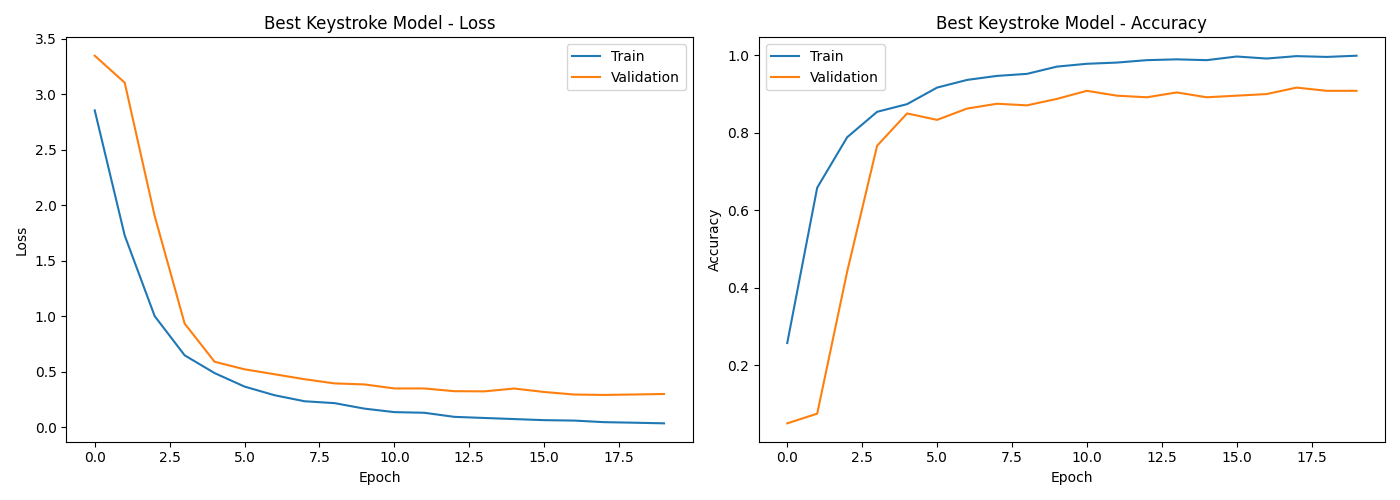
\includegraphics[width=0.9\linewidth]{3Lab/results/best_model/keystroke/history.png}
    \caption{Laiko eilučių geriausio modelio mokymo ir validavimo metrikos}
    \label{fig:geriausias_keystroke_history}
\end{figure}

\begin{figure}[H]
    \centering
    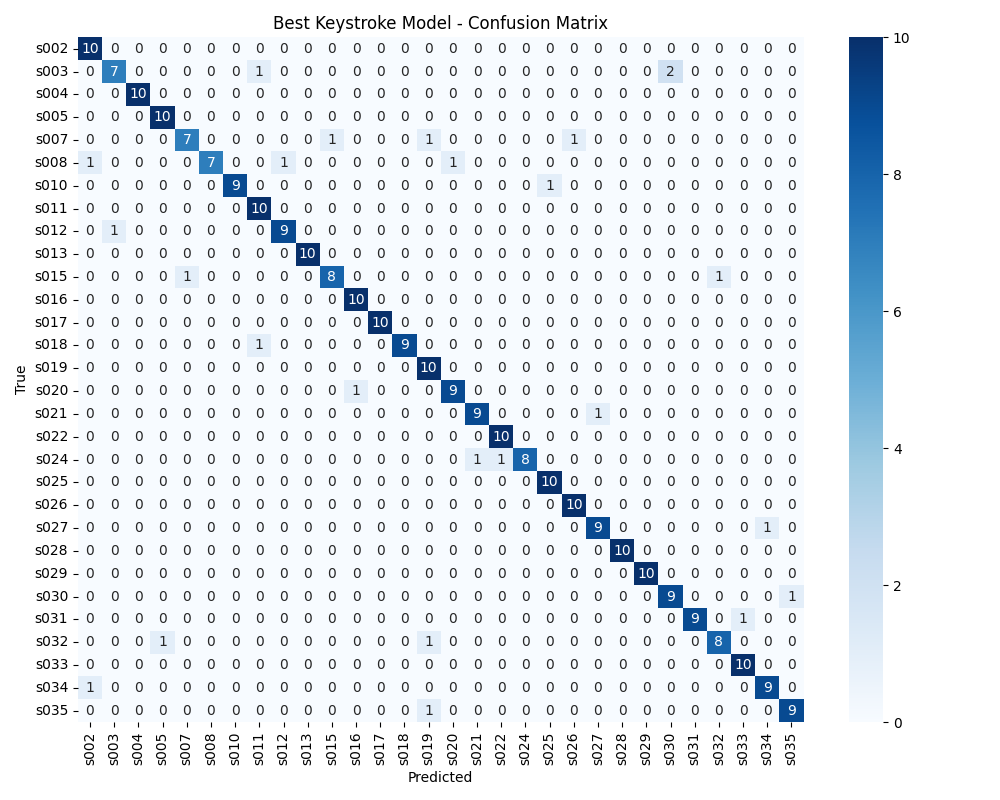
\includegraphics[width=0.95\linewidth]{3Lab/results/best_model/keystroke/confusion_matrix.png}
    \caption{Laiko eilučių geriausio modelio klasifikavimo matrica testavimo aibėje}
    \label{fig:geriausias_keystroke_cm}
\end{figure}
